% !TEX root = ../deviant-tkde.tex

\newcommand{\todoinfc}[1]{\todo[inline,backgroundcolor=yellow]{FC: #1}}



\section{Experimental evaluation}
\label{sec:eval}

% Usually, an experimental evaluation of a process discovery algorithm would require to apply the proposed approach on one (or more) dataset, and to confront the learned model with those ones mined by other available approaches. However, our approach makes explicit use of information from traces labeled as ``negative'', while the totality of the approaches we could access have been designed to use positive traces only. Hence, confronting different approaches on different input data would not be fair.
% NO, questa motivazine non va bene...

One of the difficulties of evaluating process mining algorithms is that given a log, the underlying model might not be known before. As a consequence, it might be difficult to establish an \emph{ideal model} (a golden standard) to refer and confront with. In this regard, a number of metrics and evaluation indexes have been proposed in the past to evaluate how a discovered model fits a given log \cite{2015-Adriansyah,2014-Broucke,2018-Ponce}. However, those metrics might provide only a partial answer to the question of \tcolor{blue}{``how good'' the discovered model is}. 
%
In the case of \nd, a further issue influences the evaluation process: the difficulty of performing a ``fair'' comparison with existing techniques because the majority of the methods we could access have been designed to use ``positive'' traces only.


%A second issue is about the difficulty of confronting our approach with existing ones, especially if we consider that \todofc{Non so se questa cosa la voglio scrivere qui\ldots} our approach exploits information from traces labeled as ``negative'', while the majority of the approaches we could access have been designed to use positive traces only.

We pursued two different evaluation strategies. On one side, we defined a model, and from that model we generated a synthetic, artificial log, taking care that it exhibits a number of desired properties: in a sense, this part of the evaluation can be referred as being about a ``controlled setting''. A first aim is to understand if \nd succeeds to discover a \emph{minimum} set of constraints for distinguishing positive from negative examples; a second aim is to qualitatively evaluate the discovered model, having the possibility to confront it with the original one. Experiments conducted on that synthetic log are reported and discussed in Section \ref{sec:syntheticlog}.

On the other side, we applied \nd to some existing logs, thus evaluating it on some real data set. Again, this experiment has two aims: to understand weakness and strengths of \nd w.r.t. to some relevant literature; and to confront the proposed approach with real-world data---and difficulties that real-world data bring along. Section \ref{sec:realdata} is devoted to present the selected logs and discuss the obtained results.

The source code and the experiments are available in~\cite{negdis:2021_5158528}.

% Such aspect is further exacerbated by the fact that our approach exploits information from traces labeled as ``negative'', while the totality of the approaches we could access have been designed to use positive traces only.



\subsection{Experiments on a synthetic dataset}
\label{sec:syntheticlog}

% PER REFERENCE INTERBA NOSTRA:
%
% init(receive_loan_application)
% existence(assess_eligibility)
% precedence(assess_loan_risk, assess_eligibility)
% precedence(appraise_property, assess_eligibility)
% exclusive_choice(reject_application, send_acceptance_pack)
% precedence(assess_eligibility, reject_application)
% precedence(assess_eligibility, send_acceptance_pack)
% not_coexistence(reject_application, notify_approval)
% not_coexistence(receive_positive_feedback, receive_negative_feedback)
% exclusive_choice(send_acceptance_pack, receive_negative_feedback)
% precedence(appraise_property, assess_loan_risk)

% existence(0, 1, appraise_property)
% existence(0, 1, check_credit_history)
% existence(0, 1, check_income_sources)
% existence(0, 1, assess_loan_risk)
% , assess_eligibility % rimosso perché è già oggetto di un vincolo existence...
% existence(0, 1, reject_application)
% existence(0, 1, send_acceptance_pack)
% existence(0, 1, verify_receipt)
% existence(0, 1, cancel_application)
% existence(0, 1, notify_cancellation)
% existence(0, 1, approve_application)
% existence(0, 1, notify_approval)
% existence(0, 1, ask_for_customer_feedback)
% existence(0, 1, receive_positive_feedback)
% existence(0, 1, receive_negative_feedback)

The synthetic log has been generated starting from a Declare model, using a tool \cite{2020-Loreti} based on Abductive Logic Programming. The model has been inspired by the Loan Application process reported in \cite{DBLP:books/sp/DumasRMR18}. In our model, the process starts when the \emph{loan application} is received. Before \emph{assessing the eligibility}, the bank proceeds to \emph{appraise the property} of the customer, and to \emph{assess the loan risk}. Then, the bank can either \emph{reject the application} or \emph{send the acceptance pack} and, optionally, \emph{notify the approval} (if not rejected). During the process execution the bank can also \emph{receive positive} or \emph{negative feedback} (but not both), according to the experience of the loan requester. It is not expected, however, that the bank receives a \emph{negative feedback} if the \emph{acceptance pack} has been sent. Moreover, due to temporal optimisation, the bank requires that the \emph{\tcolor{blue}{appraisal }of the property} is done before \emph{assessing the loan risk}.
To ease the understanding of the loan application process, a Declare model of the process is reported in Fig. \ref{fig:ex}. Moreover, all the activities have been constrained to either not be executed at all, or to be executed at most once: in Declare terminology, all the activities have been constrained to $\mathsf{absence2(X)}$.

\begin{figure}[t]
\centering
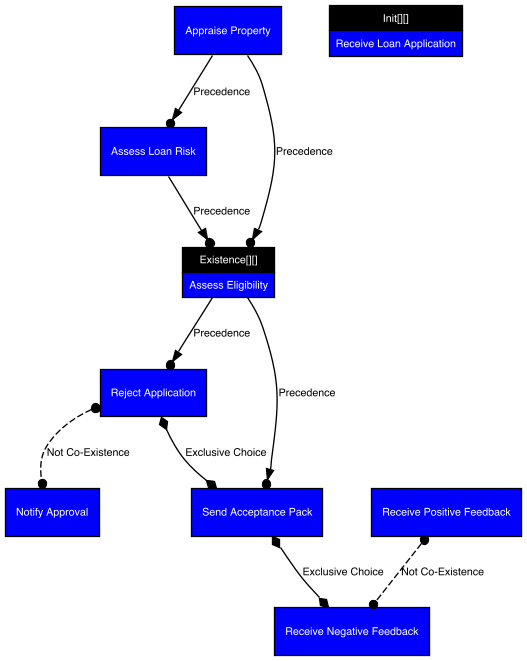
\includegraphics[width=0.6\columnwidth]{example1}
\caption{Loan approval declare process model.}
\label{fig:ex}
\end{figure}

To test \nd, besides positive traces, we generated also negative traces. In particular, we generated traces that violate two different constraints:
% \todofc{Non ho messo il terzo test di violazione, perch\`e riguardava ancora una \emph{precedence}\ldots pensiamo se vogliamo aggiungerlo.}
\begin{enumerate}[label=(\textit{\alph*})]
\item the $\mathsf{precedence(assess\_loan\_risk, assess\_eligibility)}$, that is violated when either the latter activity is executed and the former is absent, or if both the activities appear in the log, but in the wrong temporal order;
%
\item the $\mathsf{exclusive\_choice(send\_acceptance\_pack}$, $\mathsf{receive\_negative\_feedback)}$, that is violated when a trace either contains both the activities, or does not contain any of them.
\end{enumerate}
%
The resulting log consists of 64,000 positives traces, 25,600 traces that violate the constraint as in $(a)$, and 10,240 traces that violate the constraint as specified in $(b)$.
%
When fed with the positives traces and traces violating the constraint in $(a)$, \nd successfully manages to identify constraints that allow to clearly distinguish \tcolor{blue}{positive/negative }traces. Moreover, the discovered constraint coincides with the one we originally decided to violate during the generation phase. When confronted with the scenario $(b)$, \nd again successfully managed to identify a minimum model able to discriminate between positive and negative traces, and the identified constraint is indeed logically consistent with the constraint originally selected for the violation.
% In particular, it is worthy to notice that our approach derived 
Table \ref{tab:syntResults} summarize the obtained results and reports the first selected model for each scenario.

% source of this data:
% file:///Users/federico/Google%20Drive/on-negative-traces/experiments/2020-07-14%20Federico/run_experiments_2020-07-30_130357_CEST.html
%\todoinfc{I tempi di calcolo riportati in tabella potrebbero non essere giusti. Chiedere a Sergio\ldots in particolare, Sergio suggeriva che per gli step \texttt{compatibles} e \texttt{choices} dovremmo prendere i tempi \texttt{user + system}; per lo step \texttt{opt} invece nel caso di minclose dovremmo prendere la \texttt{CPUtime}, mentre per la subsetclose dovremmo prendere \texttt{CPUtime * (numconstraints bigger model) } }
\begin{table*}
\scalebox{.87}{
\begin{tabular}{c c c c l l}
\toprule
Scenario & Positive Trace \# & Negative Trace \#  & Time & Originally Violated Constraint & \tcolor{blue}{Best } Discovered Model \\
\midrule
$\multirow{4}{*}{(a)}$ & \multirow{4}{*}{64,000} & \multirow{4}{*}{25,600} & \bf{Total: \fpeval{81.78 + 1.94 + 109.74 + 3.32 + 15.165}s}  \\
& & & Compatibles:  \fpeval{81.78 + 1.94}s & \emph{precedence(assess\_loan\_risk,}  & \emph{precedence(assess\_loan\_risk,} \\
& & & \textit{\sheriff}: \fpeval{(109.74 + 3.32)-(81.78 + 1.94)}s  & \emph{assess\_eligibility)} & \emph{assess\_eligibility)} \\
& & & Optimisation: 15.165s & & \\
%
\midrule
%
$\multirow{4}{*}{(b)}$ & \multirow{4}{*}{64,000} & \multirow{4}{*}{10,240} & \bf{Total: \fpeval{81.78 + 1.94 + 94.51 + 2.96 + 1.379}s} \\
& & & Compatibles:  \fpeval{81.78 + 1.94}s & \emph{exclusive\_choice(send\_acceptance\_pack,} & \emph{coExistence(reject\_application,} \\
& & & \textit{\sheriff}:  \fpeval{(94.51 + 2.96)-(81.78 + 1.94)}s  & \emph{receive\_negative\_ feedback)} & \emph{receive\_negative\_feedback)}\\
& & & Optimisation: 1.379s & & \\
\bottomrule
\end{tabular}
}
\caption{Models discovered when dealing with the synthetic data set.}
\label{tab:syntResults}
\end{table*}\tododl{Best invece di First in Table\ref{tab:syntResults}?} 

% PARAMETRI RuM usati:
% Templates: devi selezionarli tutti eccetto:
%  - not precedence
%  - not chain precedence
%  - not response
%  - not chain response
%  - not responded existence
% Constraint support: io ho provato 80,90 e 100 - qui penso che puoi vedere un po' in base ai risultati che ti escono
% Pruning types: come dicevo oggi li ho provati tutti e 4 ma secondo me e` sufficiente None.
% Vacuity detection: deve essere OFF
% Activity support filter: deve essere a 0%

For the sake of completeness, we decided to experiment also with the Process Discovery Tool of the RuM Framework\footnote{\url{https://rulemining.org/}}, that is based on the Declare Miner algorithm \cite{2018a-Maggi}. Based on the exploitation of positive traces only, Declare Miner discovers a rich model that describes as ``most exactly'' as possible the given traces. When fed with the positive traces of our artificial log, and with the \emph{coverage} parameter set to 100\% (i.e., prefer constraints that are valid for all the traces in the logs), the RuM Framework discovers a model made of 514 constraints. If the coverage is relaxed to 80\% (prefer constraints that are satisfied by at least the 80\% of the traces), the model cardinality grows up to 1031 constraints.

In both cases the discovered model is able to distinguish between the positive and the negative traces. This is not surprising, since Declare Miner aims to identify all the constraints that hold for a given log: hence, it will discover also those constraints that allow to discern positive from negative traces. Rather, this result is a clear indication that indeed our artificial log has been constructed ``correctly'', since negative traces differ from the positive ones for some specific constraints, and the positive traces exhaustively elicit the cases that can occur. 
%In a sense we could say that the log is sufficiently exhaustive of all positive cases that can occurr.Declare Miner performance are enhanced 
This is typical of artificial logs, while real-life logs might not enjoy these properties.

Another consideration is about the cardinality of the discovered model: the Declare Miner approach provides a far richer description of the positive traces, at the cost perhaps of bigger models. Our approach instead has the goal of identifying the \emph{smallest} set of constraints that allow to discriminate between positive and negatives. In this sense, approaches like the one presented in this paper and Declare Miner are complementary.

% \todoinfc{ChiaraDFM, qui ci starebbe bene un paragrafetto in cui riportiamo i risultati ottenuti usando RuM. Il commento che potremmo scrivere e' che RuM trova un modello intero per coprire le positive, e riesce a distingure benissimo anche le negative: il risultato e' atteso, dato l'elevato numero di tracce che rende il synthetic data set molto informativo.}



\subsection{Evaluation on case studies from real data}
\label{sec:realdata}

%\todoindl{Chiara DFM\&Sergio\&Fabrizio: descrizione dataset e risultati di esperimenti coi dati veri}

For the experimentation with real datasets, we used three real-life event logs: \textsc{cerv}, \textsc{sepsis} and \textsc{bpic12}. Starting from these event logs we generated 5 different datasets, each composed of a set of positive and a set of negative traces, by applying different criteria to distinguish between positive and negative traces, i.e., by labeling the event log with different labeling functions. 

\textsc{cerv} is an event log related to the process of cervical cancer screening carried out in an Italian cervical cancer screening center~\cite{2007b-Lamma}. Cervical cancer is a disease in which malignant (cancer) cells form in the tissues of the cervix of the uterus. The screening program proposes several tests in order to early detect and treat cervical cancer. It is usually composed by five phases: Screening planning; Invitation management; First level test with pap-test; Second level test with colposcopy, and eventually biopsy. The traces contained in the event log have been analyzed by a domain expert and labeled as compliant (positive traces) or non-compliant (negative traces) with respect to the cervical cancer screening protocol adopted by the screening center.

\textsc{sepsis}~\cite{Sepsis} is an event log that records trajectories of patients with symptoms of the life-threatening sepsis condition in a Dutch hospital.
%Œ\textsc{Sepsis} is an event log that records trajectories of patients with symptoms of the life-threatening sepsis condition in a Dutch hospital. 
Each case logs events since the patient's registration in the emergency room until her discharge from the hospital. Among others, laboratory tests together with their results are recorded as events. The traces contained in the event log have been labelled based on their cycle execution time. In the \textsc{sepsis$_{mean}$} dataset, traces with a cycle time lower than the mean duration of the traces in the event log (\textasciitilde\xspace28 days) have been labelled as positive, as negative otherwise. Similarly, in the \textsc{sepsis$_{median}$}, traces with a cycle time lower than the median duration of the traces in the event log (\textasciitilde\xspace 5 days)  have been labeled as positive; as negative otherwise.  

\tcolor{blue}{\textsc{bpic12} is a real-life event log from the Business Process Intelligence Challenge of 2012 ~\cite{BPIC2012}. It pertains to the application process for personal loans or overdrafts in a Dutch financial institute}. It merges three intertwined sub-processes. Also in this case, the traces have been labelled based on their cycle execution time. In the \textsc{bpic12$_{mean}$} dataset (resp. \textsc{bpic12$_{mean}$}), traces with a cycle time lower than the mean (resp. median) duration of the traces in the event log (\textasciitilde\xspace 8 days, resp. \textasciitilde\xspace 19 hours) have been labelled as positive; as negative otherwise. 


Table~\ref{tab:rl_datasets} summarizes the data related to the five resulting datasets.

\begin{table}[h]
	\renewcommand{\arraystretch}{1.2}
	\centering
	\scalebox{0.7}{
		\begin{tabular} {l l c c c c c}
		\toprule
			\multirow{2}{*}{\textbf{Dataset}} & \multirow{2}{*}{\textbf{Log}} & \multirow{2}{*}{\textbf{Trace \#}} & \multirow{2}{*}{\textbf{Activity \#}} & \multirow{2}{*}{\textbf{Label}} & \textbf{Positive} & \textbf{Negative}  \\ 
			& & & & & \textbf{Trace \#} & \textbf{Trace \#} \\ \midrule
			\textsc{cerv$_{compl}$} & \textsc{cerv} & 157 & 16 & compliant & 55 & 102 \\ \midrule
			\textsc{sepsis$_{mean}$} & \multirow{2}{*}{\textsc{sepsis}} & \multirow{2}{*}{1000} & \multirow{2}{*}{16} & mean duration & 838 & 212 \\
			\textsc{sepsis$_{median}$} &  &  &  & median duration & 525 & 525 \\ \midrule
			\textsc{bpic12$_{mean}$} & \multirow{2}{*}{\textsc{bpic12}} & \multirow{2}{*}{13087} & \multirow{2}{*}{36} & mean duration & 8160 & 4927  \\
			\textsc{bpic12$_{median}$} &  &  &  & median duration & 6544  & 6543 \\ 			
			\bottomrule
		\end{tabular}}
		\caption{Dataset description}
		\label{tab:rl_datasets}
\end{table}

The results obtained by applying the \nd algorithm are summarised in Table~\ref{tab:rl_results}. The table reports for each dataset, the results related to the \subsetclos (connected to the \emph{generality} criterion of Eq. \ref{eq:most-gen} and \ref{eq:redun}) and \minclos (\emph{simplicity} criterion of Eq. \ref{eq:simpl1} and \ref{eq:simpl2}) optimizations in terms of number of returned models\footnote{We stop generating models after $20$ models, i.e., \para{max} in Table~\ref{tab:rl_results} indicates that more than $20$ models have been returned.}, minimum size of the returned models, as well as percentage of negative traces violated by the returned model. Moreover, the table reports the time required for computing the set of compatibles, the set of \sheriff, as well as the \subsetclos and \minclos optimizations.

\begin{table*} [h]
	\renewcommand{\arraystretch}{1.2}
	\centering
	\scalebox{0.7}{
		\begin{tabular} {l c c c  c c c c c c c}
		\toprule
			\multirow{4}{*}{\textbf{Dataset}} & \multicolumn{3}{c}{\textbf{\subsetclos}} &  			\multicolumn{3}{c}{\textbf{\minclos}}  & 	\multicolumn{4}{c}{\textbf{ Required Time (s)}} \\ 
			\cmidrule(r){2-4} \cmidrule(r){5-7} \cmidrule(r){8-11}
			& \textbf{Number of} & \textbf{Min model} & \textbf{Violated} & \textbf{Number of } & \textbf{Min model} & \textbf{Violated} & \multirow{2}{*}{\textbf{Comp.}} & \multirow{2}{*}{\textbf{\textit{\sheriff}}} & \multirow{2}{*}{\textbf{\subsetclos}} & \multirow{2}{*}{\textbf{\minclos}}  \\			
			& \textbf{models} & \textbf{size} & \textbf{$L^{-}$ trace \%} & \textbf{models} & \textbf{size} & \textbf{$L^{-}$ trace \%} & & & & \\ \midrule
			 \textsc{cerv$_{compl}$} & \para{max} & 4 & 100\% & \para{max} & 4 & 100\% & 0.12 & 0.21 & 0.065 & 0.045\\ \midrule
			\textsc{sepsis$_{mean}$} & 1 & 8 & 4.25\% & 1 & 8  & 4.25\% & 0.73 & 0.31 & 0.039 & 0.035\\ 
			\textsc{sepsis$_{median}$} & \para{max} & 14 & 26.86\% & 16 & 14 & 26.86\% & 0.45 &	1.05 & 0.2 & 0.087 \\ \midrule
			\textsc{bpic12$_{mean}$} & \para{max} & 12 & 1.42\% & \para{max} & 12 & 1.42\% & 13.51 & 17.49 & 0.096 & 0.066  \\ 
			\textsc{bpic12$_{median}$} & \para{max} & 23 & 36.59\% & \para{max} & 22 & 36.59\% & 13.32 & 24.31 & 359.164 & 43.846 \\ 			
			\bottomrule
		\end{tabular}}
		\caption{\nd results on the real-life logs}
		\label{tab:rl_results}
\end{table*}

The table shows that for the \textsc{cerv$_{compl}$} dataset, \nd is able to return models that satisfy the whole set of positive traces and violate the whole set of negative traces (the percentage of violated traces in $L^-$ is equal to 100\%) with a very low number of constraints (4). For the other datasets, the returned models are always able to satisfy all traces in $L^+$, however not all the negative traces are violated by the returned models. In case of the datasets built by using the mean of the trace cycle time, the percentage of violated traces is relatively small ($4.25\%$ for \textsc{sepsis$_{mean}$} and $1.24\%$ for \textsc{bpic12$_{mean}$}), as the number of constraints of the returned models ($8$ for \textsc{sepsis$_{mean}$} and $12$ for \textsc{bpic12$_{mean}$}). Nevertheless, \nd is able to obtain reasonable results with the real life datasets built with the median of the trace cycle time. Indeed, it is able to identify $14$ (resp. $22$-$23$) constraints able to accept all traces in $L^+$ and to cover about $27\%$ (resp. $37\%$) of the traces in $L^-$ for \textsc{sepsis$_{median}$} (resp. \textsc{bpic12$_{median}$}). The difference in terms of results between the \textsc{cerv$_{compl}$} and the other datasets is not surprising. Indeed, while what characterizes positive and negative traces in the \textsc{cerv$_{compl}$} dataset depends upon the control flow (i.e., it depends on whether each execution complies with the cervical cancer screening protocol adopted by the screening center), when mean and median cycle time are used, the difference between positive and negative traces could likely not exclusively depend upon the control flow of the considered traces. Overall, the inability to identify a set of constraints that is able to fulfil all traces  in $L^+$ and to violate all negative ones is due to a bias of the considered language (Declare without data) that does not allow to explain the positive traces without the negative ones.

The difference of the results obtained with the mean and the median cycle time can also be explained as a language bias issue for the specific labelled datasets. Indeed, while when the positive and negative trace sets are quite balanced (i.e., for \textsc{sepsis$_{median}$} and \textsc{bpic12$_{median}$}) \nd is able to identify a set of constraints (related to the control flow) describing the traces with a low-medium cycle time and excluding the ones with a medium-high cycle time, when the sets of the positive and the negative traces are quite imbalanced (i.e., for \textsc{sepsis$_{mean}$} and \textsc{BPIC12$_{mean}$})
%(the size of the set of the positive traces is about 4 times, resp. 2 times, the size of the set of the negative traces in \textsc{sepsis$_{mean}$} and \textsc{BPIC12$_{mean}$}, respectively)
 characterizing the high number of traces with a low or medium cycle time while excluding the ones with a very high cycle time can become hard. 

The table also shows that \nd is overall very fast for small datasets (e.g., less than one minute for \textsc{cerv$_{compl}$}), while it requires some more time for large ones (e.g., \textsc{bpic12$_{mean}$} and \textsc{bpic12$_{median}$}). While the time required for computing \textit{compatibles} and \textit{\sheriff} seems to be related to the size of the dataset, the time required for computing the optimizations seems to depend also on other characteristics of the datasets. 

%We compared the obtained results with the ones obtained with state-of-the-art techniques for the discovery of declarative models starting (i) from  only positive traces; and (ii) from both positive and negative traces. 

%For the former case, we used the state-of-the-art Declare miner algorithm~\cite{2018a-Maggi}  implemented in the RuM toolkit~\cite{2020-Alman}. For the latter we compared the results obtained with \nd with the ones of DecMiner, the approach based on Inductive Logic Programming proposed in~\cite{2007b-Lamma}.

Compared to state-of-the-art techniques for the discovery of declarative models starting from the only positive traces, \nd is able to return a small number of constraints satisfying all traces in $L^+$ without decreasing the percentage of violated traces in $L^-$.  
%Concerning the classical declarative discovery from only positive execution traces, 
Among the classical declarative discovery approach, we selected the state-of-the-art \declareminer algorithm~\cite{2018a-Maggi} implemented in the \rum toolkit~\cite{2020-Alman}. We discovered the models using the only positive traces and setting the \para{support} parameter, which measures the percentage of (positive) traces satisfied by the \declare model, to 100\%\footnote{We run the \declareminer algorithm with vacuity detection disabled, \para{activity support filter} set to 0\%, using both transitive closure and hierarchy-based reduction of the discovered constraints, as well as with the whole set of Declare templates.}.
%We used the \declareminer algorithm\footnote{We run the \declareminer algorithm with vacuity detection disabled, \par{activity support filter} set to 0\%, using both transitive closure and hierarchy-based reduction of the discovered constraints, as well as with all the Declare templates, except for \dec{NotResponse}, \dec{NotPrecedence}, \dec{NotChainPrecedence}, \dec{NotChainResponse}, \dec{NotRespondedExistence}.} to discover the \declare model starting from the only positive traces with different values of the \para{support} parameter, which measures the percentage of (positive) traces satisfied by the \declare model.  \todocdf{Move this part when the results are presented for the synthetic data}

Table~\ref{tab:rl_declare_miner} summarises the obtained results\footnote{Note that the results obtained with DeclareMiner and NegDis are not fully comparable. Indeed, the discovery mechanisms behind the two tools are different, and different is even the information that the tools take as input. DeclareMiner takes as input only the positive log and bases the discovery on the positive log alphabet. Instead, NegDis uses information from both positive and negative logs, including the alphabet of the discovered model that, in general, is not the same as the one retrieved from the positive log only.
}. The table reports for each dataset, the size of the model in terms of number of constraints, as well as the percentage of negative traces violated by the model. For lower values of the \para{support} parameter, i.e., for a lower percentage of positive traces satisfied by the model, the model returned by the \declareminer violates a higher percentage of negative traces. In this way, the \para{support} parameter allows for balancing the percentage of positive trace satisfied and negative traces violated. 

As hypothesised, the optimisation mechanism in \nd is able to identify a small set of constraints, that guarantees the satisfaction of all traces in $L^+$ and the same percentage of negative trace violations obtained with \declareminer (with \para{support} to 100\%).

%\begin{table} [ht]
%	\centering
%	\scalebox{0.8}{
%		\begin{tabular} {l c c}
%		\toprule
%			\textbf{Dataset} & \textbf{Model size} & \textbf{Violated L$^{-}$ trace \%}  \\ \midrule
%			\textsc{cerv$_{compl}$} & 323 & 100\% \\ \midrule
%			\textsc{sepsis$_{mean}$} & 210 & 4.25\%\\ 
%			\textsc{sepsis$_{median}$} & 202 & 26.86\% \\ \midrule
%      \textsc{bpic12$_{mean}$} & 514 & 1.42\% \\ 
%			\textsc{bpic12$_{median}$} & 532 & 36.59\% \\ 
%		\bottomrule
%		\end{tabular}}
%		\caption{\declareminer results}
%		\label{tab:rl_declare_miner}
%\end{table}
\begin{table} [ht]
	\centering
	\scalebox{0.8}{
		\begin{tabular} {l c c}
		\toprule
			\textbf{Dataset} & \textbf{Model size} & \textbf{Violated L$^{-}$ trace \%}  \\ \midrule
			\textsc{cerv$_{compl}$} & 323 & 100\% \\ \midrule
			\textsc{sepsis$_{mean}$} & 213 & 4.25\%\\ 
			\textsc{sepsis$_{median}$} & 203 & 22.29\% \\ \midrule
      \textsc{bpic12$_{mean}$} & 515 & 0.91\% \\ 
			\textsc{bpic12$_{median}$} & 532 & 32.7\% \\ 
		\bottomrule
		\end{tabular}}
		\caption{\declareminer results}
		\label{tab:rl_declare_miner}
\end{table}

Finally, we evaluated the results obtained with \nd relying on the same procedure and dataset (\textsc{cerv$_{compl}$}) used in ~\cite{2007b-Lamma} to assess the results of \decminer, a state-of-the-art declarative discovery approach based on Inductive Logic Programming that is able to use both positive and negative execution traces. 
%To this aim, we run the same procedure described in~\cite{2007b-Lamma} on the same dataset (the \textsc{cerv$_{compl}$} dataset) used in the same paper. 
Five fold-cross validation is used, i.e., the \textsc{cerv$_{compl}$} dataset is divided into 5 folds and, in each experiment, 4 folds are used for training and the remaining one for validation purposes. The average \emph{accuracy} of the five executions is collected, where the accuracy is defined as the sum of the number of positive (compliant) traces that are (correctly) satisfied by the learned model and the number of negative (non-compliant) traces that are (correctly) violated by the learned model divided by the total number of traces. 
%\begin{equation*}
% accuracy = (|satisifed L^+ | + |violated L^-|)/ |L^+ + L^-|
%\end{equation*}
\begin{table} [b]
	\centering
	\scalebox{1}{
		\begin{tabular} {l c}
			\toprule
			\textbf{Approach} & \textbf{Accuracy} \\ \midrule
			 \decminer &  97.44\%\\ 
			 \declareminer & 96.79\%\\ 
			 \nd (\subsetclos) & 97.38\% \\ 			
			 \nd (\minclos) & 97.57\% \\ 
			\bottomrule
		\end{tabular}}
		\caption{Accuracy results obtained with \declareminer, \decminer and \nd}
		\label{tab:acc_results}
\end{table}

Table~\ref{tab:acc_results} reports the obtained accuracy values for the \decminer, the \declareminer (with the \para{support} parameter set to 100\%) and the \nd (both for the \minclos and \subsetclos optimization) approach. The table shows that on this specific dataset, \nd and \decminer have very close performance (with \nd \minclos performing slightly better). \declareminer presents instead on average a slightly lower accuracy mainly due to the highly constrained discovered model that, on one hand, allows for violating all negative traces in the validation set, and, on the other hand, leads to the violation of some of the positive traces in the validation set.




